%-----------------------------------------------------------------------------%
\chapter{\babDua}
%-----------------------------------------------------------------------------%
Bagian ini menjelaskan teori-teori yang digunakan dalam penelitian. Teori yang dimaksud adalah pengetahuan yang terkait dengan pelaksanaan penelitian.

%-----------------------------------------------------------------------------%
\section{Deep Learning}
%-----------------------------------------------------------------------------%
\deeplearning merupakan algoritma \ml yang dalam prosesnya memanfaatkan arsitektur \nn. Cara kerja arsitektur ini terinspirasi oleh struktur otak manusia yang tersusun dari neuron-neuron. Berbeda dengan Artificial Neural Network biasa, arsitektur Neural Network pada Deep Learning memiliki struktur yang lebih kompleks. Ide utama dari Deep Learning adalah bagaimana komputer dapat belajar dari pengalaman dengan cara melatih \nn menggunakan data-data yang berjumlah besar. \deeplearning merupakan salah satu bentuk dari \textit{Supervised Learning} yang berarti \nn dilatih menggunakan data yang telah diketahui labelnya. \nn yang telah dilatih dapat digunakan untuk menentukan label atau skor dari data-data baru. Akurasi dari nilai yang dikeluarkan bergantung pada jenis arsitektur dan data-data yang digunakan untuk melatih \nn tersebut. Dalam Deep Learning terdapat berbagai macam arsitektur yang dapat digunakan pada berbagai macam keperluan prediksi label atau skor. Beberapa jenis arsitektur yang populer adalah Deep Neural Network, Convolutional Neural Network, dan Recurrent Neural Network. Deep Neural Network.

Deep Neural Network (DNN) merupakan jenis arsitektur Deep Learning yang paling sederhana. DNN merupakan \nn yang terdiri dari satu input layer, satu atau lebih hidden layer, dan satu output layer. Layer-layer pada arsitektur ini merupakan fully connected layer dimana setiap layer tersusun dari node-node yang masing-masing terhubung dengan masing-masing node dari layer-layer tetangganya. Gambar menunjukkan contoh arsitektur DNN.

\begin{figure}
	\centering
	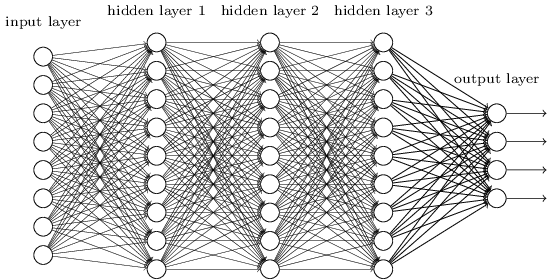
\includegraphics[width=0.50\textwidth]
	{pics/dnn.png}
	\caption{Contoh Arsitektur Deep Neural Netowork.}
	\label{fig:dnn}
\end{figure}

Karena arsitekturnya yang sederhana, DNN pada banyak kasus memiliki performa yang tidak sebaik arsitektur-arsitektur lain. DNN lebih tepat digunakan untuk melakukan tugas-tugas prediksi sederhana yang fitur-fitur dari data yang akan diprediksi sudah diketahui.

Convolutional Neural Network (CNN) merupakan arsitektur \deeplearning yang sering digunakan dalam bidang pengolahan citra. CNN pada umumnya terdiri dari beberapa convolution layer, pooling layer, dan fully-connected layer. Convolution layer dan Pooling layer merupakan beberapa jenis layer pada arsitektur ini yang tidak terdapat pada arsitektur-arsitektur lain. Convolution layer biasanya berfungsi untuk mengekstrak fitur-fitur dari data dua dimensi atau tiga dimensi yang masuk. Sedangkan pooling layer berfungsi mereduksi ukuran data output dari convolution layer dengan cara melakukan sampling terhadap data tersebut. Fully-connected layer diletakkan pada akhir arsitektur yang memiliki fungsi untuk melakukan prediksi, sama seperti DNN, dengan menggunakan fitur-fitur hasil ekstraksi convolution layer. Gambar merupakan contoh arsitektur CNN.

\begin{figure}
	\centering
	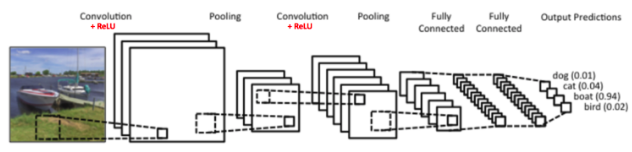
\includegraphics[width=0.50\textwidth]
	{pics/cnn.png}
	\caption{Contoh Arsitektur \conv \nn.}
	\label{fig:cnn}
\end{figure}


Recurrent Neural Network (RNN) merupakan arsitektur Deep Learning yang dapat memproses data yang bersifat sekuensial. Arsitektur ini terdiri dari input layer, hidden layer, dan output layer yang mengandung loop, dimana hasil prediksi dari output layer pada suatu waktu digunakan untuk mengubah parameter dari layer-layer sebelumnya untuk melakukan prediksi pada waktu berikutnya. Dapat dikatakan bahwa output dari suatu layer pada suatu waktu bergantung pada output dari layer itu sendiri pada waktu-waktu sebelumnya. Gambar merupakan contoh arsitektur RNN.

\begin{figure}
	\centering
	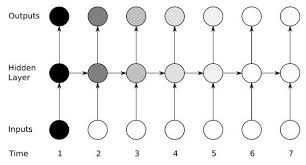
\includegraphics[width=0.50\textwidth]
	{pics/rnn.jpeg}
	\caption{Contoh Arsitektur Recurrent Neural Netowork.}
	\label{fig:rnn}
\end{figure}

RNN sangat populer dalam bidang Natural Language Processing (NLP) karena kemampuannya mengolah bahasa baik berupa audio atau teks. Hal ini karena bahasa berupa teks atau audio merupakan data yang bersifat sekuensial. 

Dengan melihat contoh-contoh arsitektur \deeplearning di atas, sekilas dapat diketahui bahwa Deep Learning memiliki beban komputasi yang cukup besar, terutama pada CNN, karena melibatkan banyak parameter dan banyak layer. Oleh karena itu, penggunaan CPU saja dirasa kurang cukup dalam menjalankan operasi-operasi pada Deep Learning.
%-----------------------------------------------------------------------------%
\section{Deep Learning Training dan Inference}
%-----------------------------------------------------------------------------%
Sama seperti \nn biasa, arsitektur \nn dalam Deep Learning memiliki parameter \weight pada setiap layer yang digunakan untuk menghitung skor dari input yang masuk ke suatu \layer dan meneruskan hasilnya ke \layer berikutnya. Deep Learning terdiri dari dua  tahap yaitu training dan inference. Pada tahap training, model \nn dilatih menggunakan sekumpulan data. Dalam hal ini yang dilatih adalah parameter \weight hingga menemukan parameter yang optimal.

Untuk mengawali proses \training, \weight awal diberikan terlebih dahulu kepada model. Biasanya \weight awal ini merupakan angka-angka acak berdasarkan suatu distribusi tertentu. Kemudian, model dengan \weight awal yang belum optimal tersebut digunakan untuk melakukan prediksi label atau skor dari data dengan melakukan \textit{forward pass} sepanjang model dari \layer pertama (input \layer) hingga mencapai \layer terakhir (\outputa \layer).

Hasil prediksi kemudian dibandingkan dengan label aslinya. Nilai \error dari prediksi dapat dihitung menggunakan fungsi tertentu, misalnya \textit{Mean Square Error}. Informasi \error ini kemudian dikirim kembali ke \layer-\layer sebelumnya dan akan digunakan oleh \layer-\layer terebut untuk memperbarui parameter \weight yang belum optimal tadi berdasarkan informasi \error yang diterima. \textit{Weight} dapat diperbarui menggunakan algoritma atau fungsi pembaruan \weight tertentu. Proses prediksi dan mengembalikan \error ke belakang ini disebut \textit{back propagation}. 

Setelah \training selesai, model \nn dapat digunakan untuk melakukan proses \inference. Tahap \inference merupakan tahap dimana model yang telah dilatih digunakan untuk melakukan prediksi. Proses prediksi ini sama dengan prediksi ketika melakukan \training yaitu dengan melakukan \textit{forward-pass} terhadap input data mulai dari \inputa \layer hingga \outputa \layer pada model. 

Letak perbedaan proses \inference dan \training pada \deeplearning adalah pada tahap \textit{back-propagation}. Setelah melakukan prediksi pada proses \inference , tidak lagi dilakukan \textit{back-propagation} terhadap \error hasil prediksi seperti pada proses \training. Hal ini karena tujuan dari \inference adalah mendapatkan hasil prediksi skor atau label yang dikeluarkan oleh model yang telah dilatih. Gambar 2.1 menunjukkan perbedaan proses \training dan \inference pada \nn . Terlihat bahwa \training melakukan pemrosesan data pada dua arah, sedangkan \inference hanya satu arah.

\begin{figure}
	\centering
	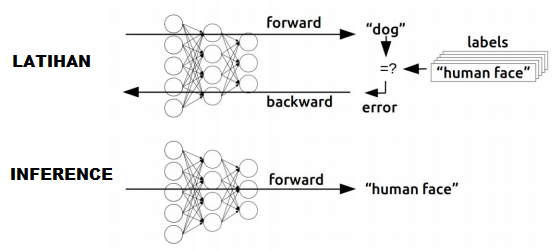
\includegraphics[width=0.50\textwidth]
	{pics/trainingvsinference.png}
	\caption{Perbedaan proses \training dan \inference pada \deeplearning.}
	\label{fig:trainvsinfer}
\end{figure}

\section{Operasi-operasi Deep Learning Inference}
%-----------------------------------------------------------------------------%
Tahap inference pada Deep Learning melibatakan banyak sekali operasi matriks yang biasanya merupakan operasi antara input data pada suatu layer dengan weight pada layer itu. Beberapa operasi bahkan memiliki kompleksitas yang tinggi. Berikut adalah beberapa contoh operasi penting yang sering muncul pada Deep Learning inference.

\subsection{Perkalian Matriks}
Operasi perkalian matriks pada Deep Learning inference merupakan salah satu operasi yang memiliki beban komputasi terbesar. Perkalian matriks dapat terjadi pada bagian fully-connected layer. Pada suatu fully-connected layer ke-l, parameter weight disimpan dalam bentuk matriks yang berukuran MxN dimana M adalah banyaknya node pada layer ke-l dan N adalah banyaknya node pada layer ke-(l-1). Baris ke-i pada weight matriks dari layer ke-l tersebut merupakan weight dari node ke-i pada layer ke-l. Untuk menentukan nilai node-node pada layer ke-l, matrix MxN tersebut dikalikan dengan matrix Nx1 yang berisi nilai-nilai node layer ke-(l-1) sehingga menghasilkan matriks Mx1. Kemudian activation function diterapkan terhadap setiap elemen matriks Mx1 tersebut dan kemudian bias juga ditambahkan jika ada sehingga menghasilkan matriks Mx1 yang merupakan nilai node-node layer ke-i. Gambar adalah ilustrasi dari operasi perkalian matriks pada fully-connected layer.

\begin{figure}
	\centering
	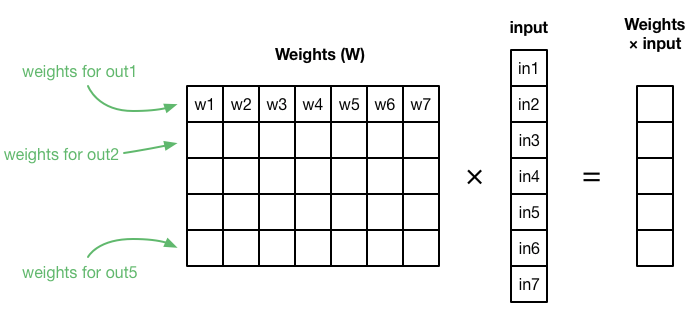
\includegraphics[width=0.50\textwidth]
	{pics/matmul.png}
	\caption{Perkalian matriks pada fully-connected layer saat mengalikan weight dengan input.}
	\label{fig:matmul}
\end{figure}

\subsection{Konvolusi Matriks}
Operasi konvolusi terjadi pada convolution layer dari CNN. Konvolusi merupakan penerapan filter atau kernel terhadap suatu input dengan mengkonvolusikan kernel tersebut terhadap input sehingga menghasilkan output. Input dan output suatu convolution layer merupakan matriks 3 dimensi yang merepresentasikan lebar, tinggi, dan kedalaman (biasa disebut channel). Sementara filter dinyatakan dalam matriks 4 dimensi yang merepresentasikan lebar filter, tinggi filter, kedalaman filter, dan banyaknya filter. Ukuran tinggi dan lebar filter selalu lebih kecil atau sama dengan tinggi dan lebar intput, sedangkan kedalamannya harus sama dengan kedalaman input.

Pada saat melakukan konvolusi terhadap input, masing-masing elemen pada suatu filter dikalikan dengan masing-masing elemen matriks input yang bersesuaian dengan posisi filter tersebut (seperti dot product pada vector) pada suatu waktu. Hasil dari satu kali operasi tersebut merupakan satu elemen dari matriks output pada posisi yang bersesuaian. Sehingga, setelah proses konvolusi selesai untuk satu filter, akan terbentuk satu lapis output dua dimensi. Jika semua filter sudah diterapkan maka akan terbentuk output tiga dimensi dengan kedalaman sesuai dengan banyaknya filter.

Gambar adalah contoh operasi konvolusi dengan input berukuran 5x5x1 dan filter berukuran 3x3x1.

\begin{figure}
	\centering
	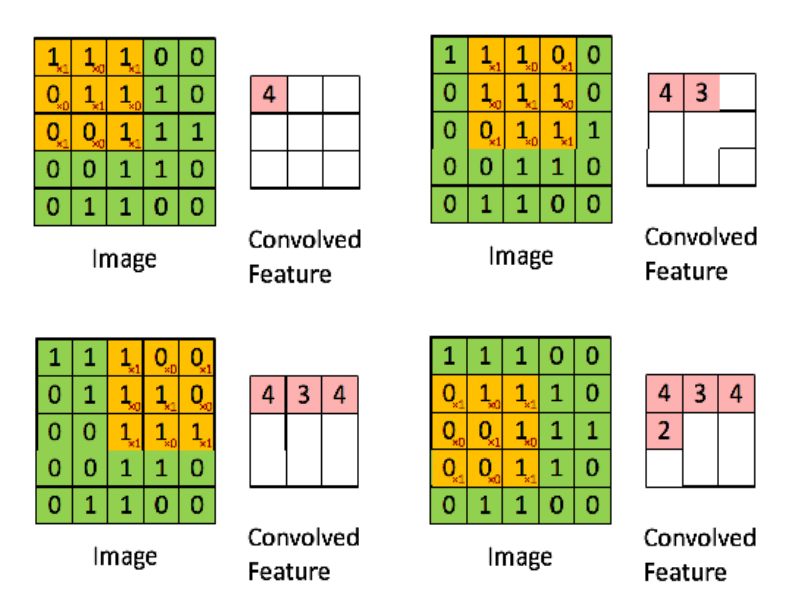
\includegraphics[width=0.50\textwidth]
	{pics/conv.png}
	\caption{Contoh Operasi Konvolusi. Image merupakan gambar masukan, convolved feature merupakan keluaran dari konvolusi.}
	\label{fig:conv}
\end{figure}

Pada operasi konvolusi dengan input berukuran MxNxD dan filter berukuran M'xN'xD' dan banyak filter adalah K, maka kompleksitas operasi konvolusi adalah O(MM'NN'DK). Operasi ini memiliki kompleksitas yang paling tinggi diantara layer-layer lain. 

\subsection{Transpose Matriks}
Transpose matriks dapat terjadi sebelum dilakukan perkalian matriks pada fully-connected layer. Operasi ini merupakan operasi membalik matriks terhadap diagonalnya. Pada matriks A dengan ukuran MxN, transpose dari A yaitu A' merupakan matriks yang tersusun dari elemen-elemen matriks A dimana A'ji = Aij untuk setiap bilangan bulat i dan j dimana 0 <= i < M dan 0 <= j < N. Gambar merupakan contoh operasi matriks transpose.

\begin{figure}
	\centering
	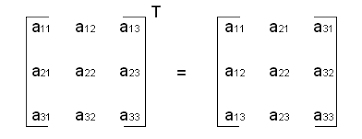
\includegraphics[width=0.50\textwidth]
	{pics/transpose.png}
	\caption{Transpose matrix pada \deeplearning \inference.}
	\label{fig:transpose}
\end{figure}

Matriks transpose memiliki kompleksitas O(MN).

\subsection{Penjumlahan Matriks}
Penjumlahan matriks dapat terjadi ketika melakukan penambahan bias terhadap hasil dari activation function suatu layer. Penjumlahan matriks dilakukan pada dua matriks berukuran sama. Pada dua matriks A dan B yang berukuran MxN, hasil penjumlahan matriks C merupakan matriks MxN dimana Cij = Aij + Bij untuk setiap bilangan bulat i dan j dimana 0 <= i < M dan 0 <= j < N. Gambar menunjukkan contoh operasi penjumlahan matriks.

\begin{figure}
	\centering
	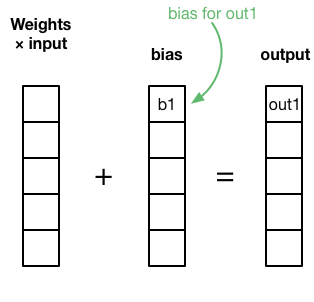
\includegraphics[width=0.50\textwidth]
	{pics/add.png}
	\caption{Penjumlahan matriks pada fully-connected layer saat menambahkan bias.}
	\label{fig:add}
\end{figure}

Pada kasus penambahan bias, lebar matriks biasanya adalah 1 atau bisa disebut sebagai vektor. Operasi ini memiliki kompleksitas O(MN), sama seperti matriks traspose.


\section{Tensorflow}
%-----------------------------------------------------------------------------%
Tensorflow merupakan perangkat lunak \textit{open-source} yang digunakan untuk komputasi numerik menggunakan representasi graf yang membentuk serangkaian operasi. Node pada graf merepresentasikan suatu operasi sedangkan edge mereperesentasikan tensor atau multidimensional array yang merupakan input atau output dari suatu operasi. Tensorflow dibuat oleh Google yang sejak awal digunakan untuk mendukung penelitian pada bidang \ml dan Deep Learning. Saat ini Tensorflow sudah sangat dikenal sebagai salah satu \framework \ml dan \deeplearning yang memiliki banyak fitur dan mudah dioperasikan. Salah satu fitur dari Tensorflow yang saat ini cukup menarik banyak perhatian adalah adanya dukungan untuk perangkat \textit{mobile} melalui \textit{library} Tensorflow Mobile dan Tensorflow Lite yang digunakan pada penelitian ini.

Tensorflow dan Tensorflow Lite diimplementasikan menggunakan bahasa C++ sehingga memungkinkan diterapkkannya OpenCL code. Kode sumber dari operasi-operasi \deeplearning \inference pada Tensorflow Lite terpisah dari kode sumber operasi-operasi \deeplearning \inference pada core Tensorflow. Modifikasi kode sumber Tensorflow Lite dengan menambahkan OpenCL code tidak akan mengubah behaviour dari program Tensorflow utama.

\section{Tensorflow Lite}
%-----------------------------------------------------------------------------%
Tensorflow Lite merupakan salah satu library dari Tensorflow yang dapat digunakan untuk proses \deeplearning \inference pada perangkat \mobile. Tensorflow sebenarnya memiliki dua \library yang dapat digunakan untuk melakukan Deep Learning \inference pada perangkat mobile, yaitu Tensorflow Mobile dan Tensorflow Lite. Tensorflow Lite memungkinkan proses inference pada perangkat mobile hanya untuk dua jenis model Neural Network yaitu Convolutional Neural Network. Tensorflow Lite, yang dirilis pada November 14, 2017, merupakan versi perbaikan dari Tensorflow Mobile yang telah dirilis terlebih dahulu.

Dalam menjalankan Deep Learning inference, Tensorflow Lite menerima input sebuah file .tflite yang berisi model dari Neural Network yang telah dilatih. Model file ini sebenarnya merupakan graph operasi Tensorflow yang berisi serangkaian node dan edge dengan ekstensi .pb namun telah dikonversi ke .tflite menggunakan Tensorflow Lite Converter. Model file tersebut diload oleh C++ API untuk kemudian diteruskan ke interpreter. API ini tersedia untuk perangkat Android maupun iOS. 

Interpreter mengeksekusi model menggunakan serangkaian kernel yang diload secara selektif, artinya hanya kernel yang berhubungan dengan operasi-operasi pada Model File saja yang diload. Ketika Tensorflow Lite dijalankan pada perangkat Android, ia akan menggunakan Android Neural Network API untuk meningkatkan performa inference. Namun tidak semua perangkat Android mendukung penggunaan Android Neural Network API. Gambar merupakan ilustrasi dari arsitektur Tensorfow Lite.

\begin{figure}
	\centering
	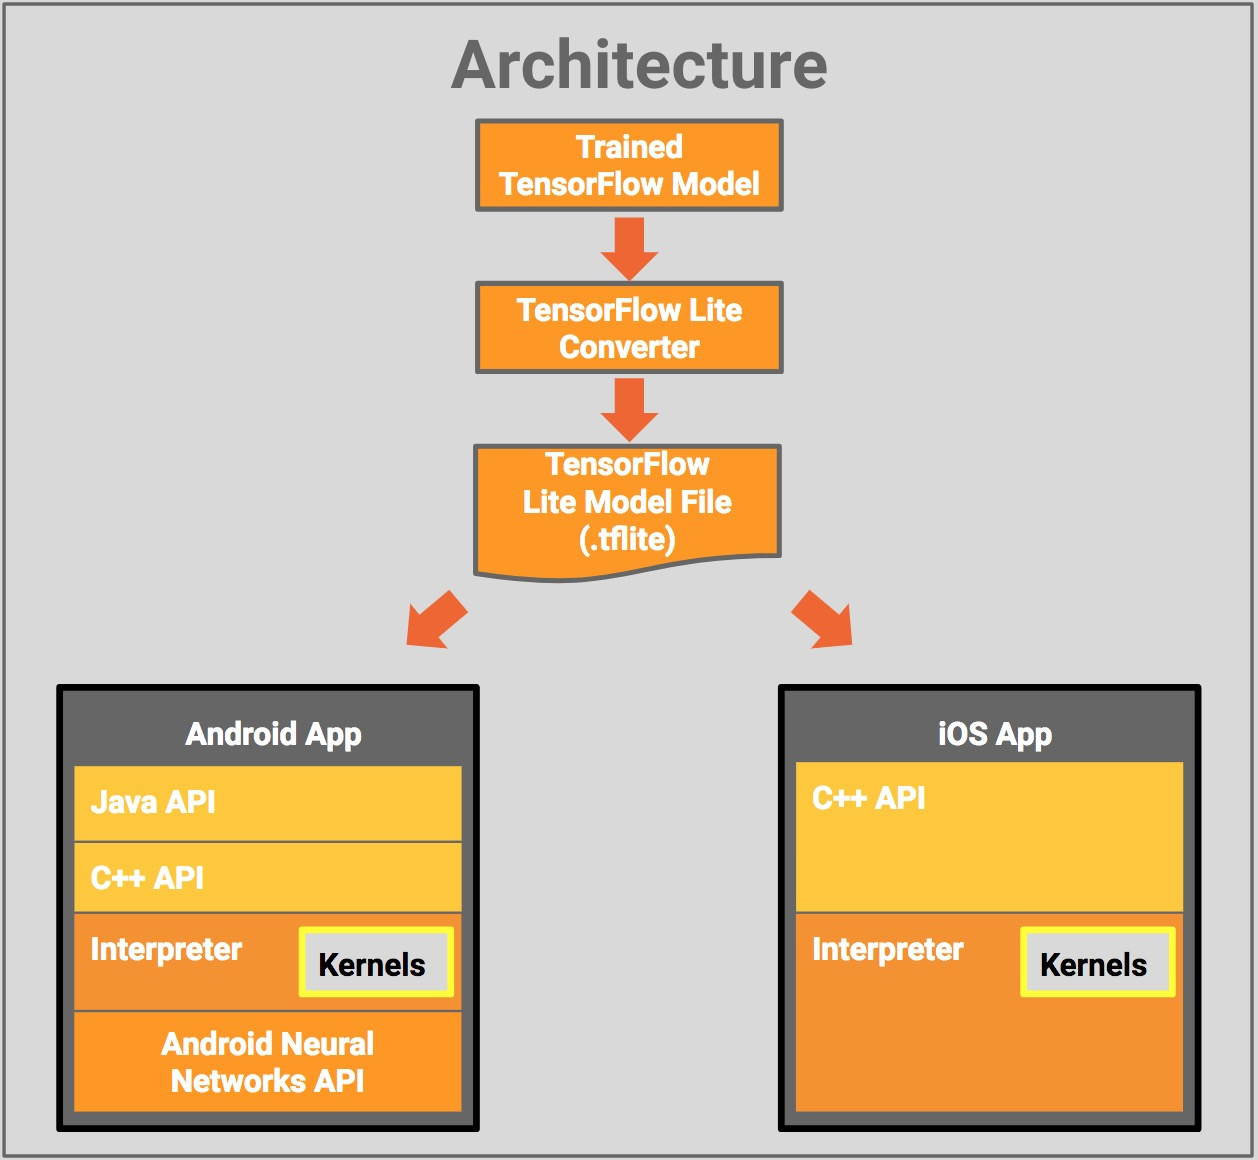
\includegraphics[width=0.50\textwidth]
	{pics/tflite.jpg}
	\caption{Ilustrasi dari arsitektur Tensorflow Lite.}
	\label{fig:tflite}
\end{figure}

Dibandingkan dengan Tensorflow Mobile, Tensorflow Lite telah mendapatkan berbagai macam optimisasi di dalamnya, sehingga memiliki performa yang lebih baik dari Tensorflow Mobile. Beberapa bug yang ada pada Tensorflow Mobile juga telah diperbaiki pada Tensorlfow Lite. Selain itu, fitur-fitur yang ditawarkan Tensorflow Lite juga lebih banyak dibandingkan Tensorflow Mobile.
Berikut adalah beberapa keunggulan Tensorflow Lite dibandingkan Tensorflow Mobile.

\begin{enumerate}
	\item Memiliki fitur yang dapat memprune node dari operation graph yang tidak terpakai pada proses inference.
	\item Memiliki kernel yang mendukung komputasi dalam 8-bit fixed point.
	\item Optimasi performa untuk operasi floating point maupun fixed point.
	\item Menggunakan pre-fused activation pada model Deep Learning.
	\item Memuat kernel secara selektif. Hanya yang terkait operasi-operasi pada model saja yang dimuat.
\end{enumerate}

\section{OpenCL}
%-----------------------------------------------------------------------------%
OpenCL merupakan antarmuka yang digunakan untuk pemrograman paralel pada prosesor yang berbeda-beda (CPU, GPU, dll) pada komputer, server, atau perangkat mobile. 
OpenCl dikenal dapat meningkatkan performa komputasi secara signifikan dengan menjalankan program secara paralel dan pada prosesor yang berbeda-beda.
Pada OpenCL terdapat dua sisi program, yaitu host dan device. Program device merupakan program yang dijalankan pada processor device yang ditargetkan (CPU, GPU, dll). Sementara itu program host berfungsi untuk mengatur jalannya program device, mulai dari menginisialisasi konteks, membuat program pada device, menyalin nilai variable dari host ke device memory, menjalankan kernel, dan mengambil nilai hasil komputasi dari device memory. Program host menggunakan bahasa C++ dengan beberapa ekstensi berupa fungsi dan tipe data khusus OpenCL.

Program yang dijalankan pada device terdiri dari satu atau lebih kernel. Kernel ditulis menggunakan bahasa C dengan sedikit perbedaan dari bahasa C biasa. Kernel pada OpenCl memiliki beberapa fungsi ekstensi dari bahasa C biasa, misalnya fungsi yang digunakan untuk mengambil worker ID dari suatu proses. 
Kernel ditulis sebagai string agar bisa digunakan oleh program host. Untuk dapat menjalankan program device, host harus terlebih dahulu membuat context. Context sendiri terbentuk dari satu atau lebih device. Contexts digunakan oleh OpenCL runtime untuk mengelola objek-objek seperti command-queues, memory, program, dan kernel. Context juga digunakan untuk mengeksekusi kernel-kernel pada satu atau lebih device yang telah terdefinisi pada context tersebut.

Setelah context terbentuk, host perlu membuat objek-objek lain seperti buffer dan command queue. Buffer merupakan bagian tertentu dari device memory yang digunakan untuk membaca atau menulis nilai yang diperlukan dalam proses kernel. Suatu buffer dapat bersifat read only, write only, atau read and write. Command queue merupakan antrian yang digunakan untuk menaruh perintah-perintah dari host kepada device. Contoh perintah adalah perintah untuk menjalankan kernel, perintah untuk menulis nilai ke buffer, dan perintah untuk membaca nilai dari buffer. Buffer dan command queue diinisialisasi pada bagian host. Gambar mengilustrasikan bagaimana OpenCL bekerja.

\begin{figure}
	\centering
	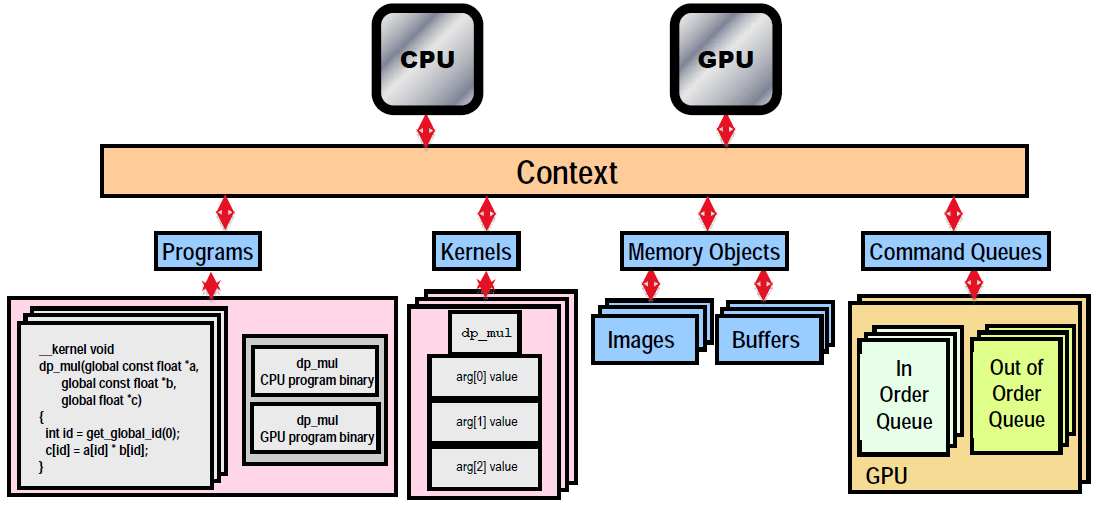
\includegraphics[width=0.50\textwidth]
	{pics/opencl-context.png}
	\caption{Cara kerja OpenCL.}
	\label{fig:context}
\end{figure}

OpenCL dapat digunakan pada perangkat yang memiliki library OpenCL, biasanya bernama libOpenCl.so. Pada NVidia GPU, library dapat diperoleh dalam paket installasi CUDA. Sedangkan pada perangkat android, beberapa vendor GPU seperti Qualcomm menyertakan library OpenCL pada perangkat mereka. Library libOpenCl.so ini biasanya terletak pada direktori /system/vendor/lib/. Berikut adalah contoh program host dan device (kernel) pada OpenCL.

\begin{lstlisting}[frame=single]
/* OpenCL Host Example */
void clHello() {
    cl_device_id device_id = NULL;
    cl_context context = NULL;
    cl_command_queue command_queue = NULL;
    cl_mem memobj = NULL;
    cl_program program = NULL;
    cl_kernel kernel = NULL;
    cl_platform_id platform_id = NULL;
    cl_uint ret_num_devices;
    cl_uint ret_num_platforms;
    cl_int ret;

    char string[MEM_SIZE];

    /* Get Platform and Device Info */
    ret = clGetPlatformIDs(1, &platform_id, 
    &ret_num_platforms);
    ret = clGetDeviceIDs( platform_id, 
    CL_DEVICE_TYPE_DEFAULT, 1, &device_id, 
    &ret_num_devices);

    /* Create OpenCL context */
    context = clCreateContext( NULL, 1, &device_id, 
    NULL, NULL, &ret);

    /* Create Command Queue */
    command_queue = clCreateCommandQueue(context, 
    device_id, 0, &ret);

    /* Create Memory Buffer */
    memobj = clCreateBuffer(context, 
    CL_MEM_READ_WRITE,MEM_SIZE * sizeof(char), NULL, 
    &ret);

    /* Create Kernel Program from the source */
    program = clCreateProgramWithSource(context, 1, 
    (const char **)&CLCL_HELLO,
    NULL, &ret);

    /* Build Kernel Program */
    ret = clBuildProgram(program, 1, &device_id, NULL, 
    NULL, NULL);

    /* Create OpenCL Kernel */
    kernel = clCreateKernel(program, "hello", &ret);

    /* Set OpenCL Kernel Arguments */
    ret = clSetKernelArg(kernel, 0, sizeof(cl_mem), 
    (void *)&memobj);

    /* Execute OpenCL Kernel */
    ret = clEnqueueTask(command_queue, kernel, 0, 
    NULL,NULL);

    /* Copy results from the memory buffer */
    ret = clEnqueueReadBuffer(command_queue, memobj, 
    CL_TRUE, 0,
    MEM_SIZE * sizeof(char),string, 0, NULL, NULL);

    /* Display Result */
    __android_log_print(ANDROID_LOG_DEBUG, "OpenCL", 
    "Hello: %s", string);


    /* Finalization */
    ret = clFlush(command_queue);
    ret = clFinish(command_queue);
    ret = clReleaseKernel(kernel);
    ret = clReleaseProgram(program);
    ret = clReleaseMemObject(memobj);
    ret = clReleaseCommandQueue(command_queue);
    ret = clReleaseContext(context);
}
\end{lstlisting}

\begin{lstlisting}[frame=single]
/* OpenCL kernel example */
const char *CLCL_HELLO =
    "__kernel void hello(__global char* string)\n"
    "{\n"
    "   string[0] = 'H';\n"
    "   string[1] = 'e';\n"
    "   string[2] = 'l';\n"
    "   string[3] = 'l';\n"
    "   string[4] = 'o';\n"
    "   string[5] = '\\0';\n"
    "}\n"
    "";
\end{lstlisting}

\section{OpenCL Data Parallelism}
%-----------------------------------------------------------------------------%
OpenCL mendukung pemrograman paralel yang dapat dilakukan pada level data maupun level device. Ketika suatu program hanya dijalankan pada satu device saja, misalnya pada penelitian ini yang hanya menggunakan rGPU sebagai OpenCL device, paralelisasi tetap dapat dilakukan pada level data. Maksudnya, data yang diproses dipecah-pecah sehingga masing-masing unit pemrosesan hanya memproses sebagian dari data secara independen terhadap unit pemrosesan lainnya. Hal ini salah satunya dapat dilakukan pada operasi matriks, misalnya pada penjumlahan matriks, penambahan elemen-elemen matriks dapat dilakukan secara paralel dengan masing-masing unit pemrosesan hanya memproses elemen pada baris dan kolom yang sama saja.

Dalam OpenCL, unit pemrosesan ini disebut dengan work item. Setiap work item melakukan hal yang sama namun hanya datanya saja yang berbeda. Dengan kata lain, setiap work item menjalankan kernel yang sama. Masing-masing work item memiliki private memory. Setiap work item juga memiliki ID masing-masing yang dapat berupa ID secara global maupun ID work item itu dalam suatu grup tertentu. ID bilangan bulat positif yang dimulai dari 0.  

Beberapa work item dapat membentuk work/local group. Proses yang terjadi pada suatu work group dapat melakukan sinkronisasi. Selain itu, work group memiliki memory tersendiri yang disebut local memory. Memory ini merupakan shared memory dimana setiap work item dalam grup dapat menggunakan local memory tersebut bersamaan. Work group juga memiliki ID seperti work item. Gambar merupakan ilustrasi dari work item dan work group pada OpenCL.

\begin{figure}
	\centering
	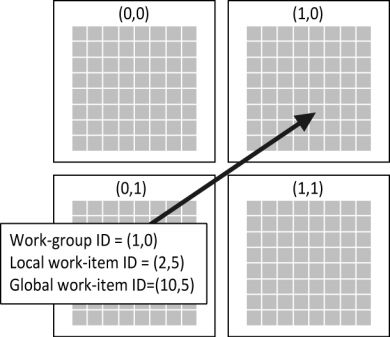
\includegraphics[width=0.50\textwidth]
	{pics/opencl-work.jpg}
	\caption{OpenCL work group dan work ite.}
	\label{fig:work}
\end{figure}

Saat suatu proses berjalan pada device, kita dapat mengambil ID dari work item atau work group yang menjalankan proses tersebut. Dengan demikian kita dapat mengatur suatu work item atau work group harus memproses bagian mana saja dari data. Misalnya dalam penjumlahan vektor, work item dengan ID i hanya memproses elemen ke i dari vektor-vektor yang dijumlahkan.